%latexmk -pdf -pvc Notes
\documentclass{article}
\setlength{\oddsidemargin}{6pt}
\setlength{\textwidth}{440pt}
\vspace{-8ex}
\usepackage{listings}
\usepackage{amsmath}
\usepackage{color}
\usepackage{graphicx}
\usepackage[left=0.70in, right=0.70in, top=0.50in, left=0.70in, headsep=0pt]{geometry}
\graphicspath{ {./assets/} }

\definecolor{dkgreen}{rgb}{0,0.6,0}
\definecolor{gray}{rgb}{0.5,0.5,0.5}
\definecolor{mauve}{rgb}{0.58,0,0.82}

\lstset{frame=tb,
  language=Java,
  aboveskip=3mm,
  belowskip=3mm,
  showstringspaces=false,
  columns=flexible,
  basicstyle={\small\ttfamily},
  numbers=none,
  numberstyle=\tiny\color{gray},
  keywordstyle=\color{blue},
  commentstyle=\color{dkgreen},
  stringstyle=\color{mauve},
  breaklines=true,
  breakatwhitespace=true,
  tabsize=3
}

\title{CMSC420 Advanced Data Structures}
\begin{document} 
  \author{Michael Li}
  \title{CMSC420 Advanced Data Structures}
  \maketitle
  \tableofcontents
  \newpage
  \noindent \section{Lists}
  \begin{lstlisting}
    init() => initializes list
    get(i) => returns element at index i
    set(i, x) => sets ith element to x
    length() => returns number of elements in the list
    insert(i, x) => insert x prior to element a_{i} (shifts indices after)
    delete(i) => deletes ith element (shift indices after)
  \end{lstlisting}
  Sequential Allocation (Array): when array is full, increase  its size but a constant factor (e.g. 2). Amortized array operations still O(1) \\ \\
  Linked Allocation (Linked List) \\ \\
  Stack(push, pop): on on end of the list \\
  Queue(enqueue, dequeue): insert at tail (end) and remove from head (start) \\
  Deque(combo stack and queue): can isnert and remove from either ends of list\\
  Multilist: multiple lists combined 1 aggregate structure (e.g. ArrayList)\\
  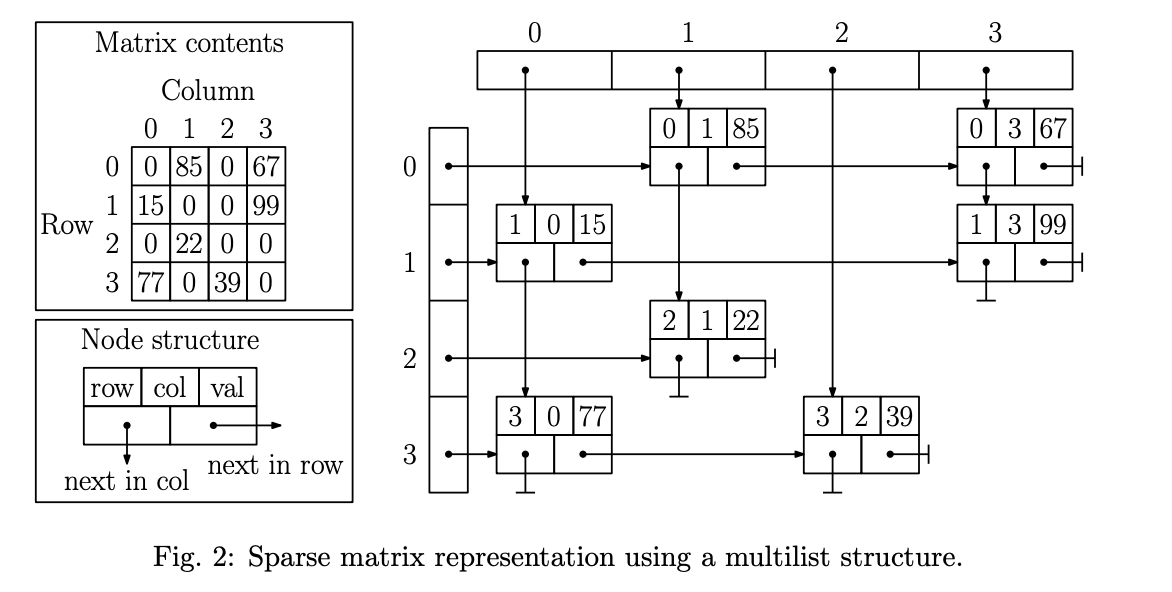
\includegraphics[width=\textwidth]{Fig_2}
  Sparse Matrix: create 2n linked lists for each row and col \\
  \indent Each entry stores a row index, col index, value, next row ptr, and next col ptr
  \newpage
  \noindent\section{Trees}
  Free Tree: connected, undirected graph with no cycles (like MST)\\
  Root Tree: each non-leaf node has $\geq$ 1 children and a single parent (except root)\\
  \indent Aborescence = out-tree \quad Anti-arborescence = in-tree \\
  \indent Depth = max \# of edges of path from root to a node \\ \\
  One way to represent tree is to have a pointer to first child and then a pointer to next sibling \\ \\
  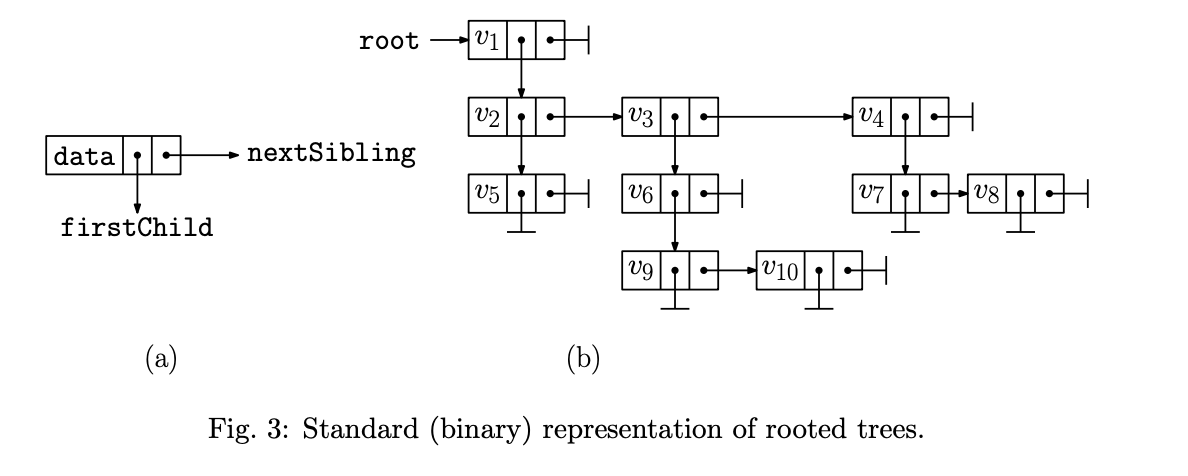
\includegraphics[width=\textwidth]{Fig_3}
  Binary Tree: rooted, ordered tree where each non-leaf node has 2 possible children (left, right) \\ 
  \indent Full Tree: All nodes either have 0 children or 2 children \\
  \indent Can make full binary tree by extending tree by adding external nodes to replace all empty subtrees\\
  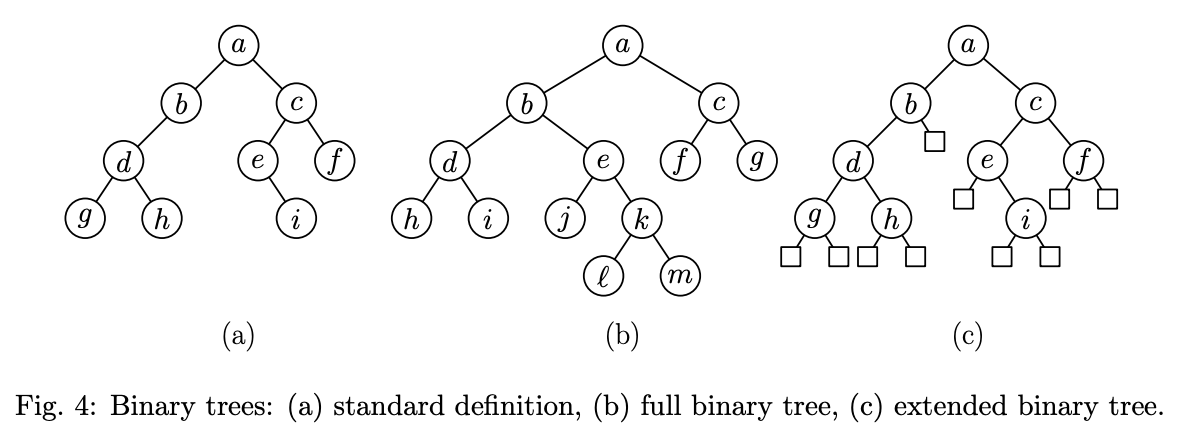
\includegraphics[width=\textwidth]{Fig_4}
  \begin{lstlisting}
    class BinaryTreeNode<E> {
      private E entry;
      private BinaryTreeNode<E> left;
      private BinaryTreeNode<E> right;
      ...
    }
  \end{lstlisting}
  In-order traversal: left, root, right \\
  Pre-order traversal: root, left, right \\ 
  Post-order traversal: left, right, root\\
  If there are n internal nodes in an extended tree, there are n+1 external nodes \\
  \indent Proof by induction: Extended tree binary tree with n internal nodes has n+1 external nodes has 2n+1 total nodes \\
  \indent Let x(n) = number of external nodes given n internal nodes and prove x(n) = n + 1 \\
  \indent Base Case x(0) = 1 a tree with no internal nodes has 1 external node \\
  \indent IH: Assume x(i) = i + 1 for all i $\leq$ n - 1 \\
  \indent IS: let $n_{L}$ and $n_{R}$ be the number of nodes in Left and Right subtrees \\
  \indent x(n) = ($n_{L}$ + 1) + ($n_{R}$ + 1) = (1 + $n_{L}$ + $n_{R}$) + 1 = n + 1 external nodes \\
  \indent so n + 1 (external) + n (internal) = 2n + 1 \\
  \indent Moreover, about 1/2 of nodes of extended Binary Tree are leaf nodes \\
  Threaded Binary Tree: Give null pointers information about where to traverse next \\
  \indent If left-child = null then stores reference to node's inorder predecessor \\
  \indent If right-child = null then stores references to node's inorder successor \\
  \includegraphics[width=\textwidth]{Fig_6}
  \begin{lstlisting}
    BinaryTreeNode inOrderSuccessor(BinaryTreeNode v) {
    BinaryTreeNode u = v.right;
    if(v.right.isThread) return u;
    while(!u.left.isThread) u = u.left;
    return u;
    }
  \end{lstlisting}
  \indent \indent if v's right-child is a thread, then we follow thread. \\
  \indent Otherwise go through v's right child and iterate through left-child links \\
  Complete Binary Tree: represented using sequential allocation (array) because no space is wasted \\
  \indent number of nodes is inbetween $2^{h}$ and $2^{h+1}-1$
  \begin{lstlisting}
    leftChild(i): if(2i <= n) then 2i else null;
    rightChild(i): if (2i + 1 <= n) then 2i + 1 else null;
    parent(i): if (i >= 2) then [i/2] else null;
  \end{lstlisting}
  \newpage
  \section{Dictionaries}
  \begin{lstlisting}
    void insert(Key x, Value v) => if key exists, exception is thrown 
    void delete(Key x) => if key does not exist, exception thrown 
    Value find(Key x) => return value associated with key or null if not found
  \end{lstlisting}
  Array representation: \\
  \indent Unsorted array has O(n) search and delete, O(1) insert although we need O(n) to check for duplicates \\
  \indent Sorted Array has O(logn) search and O(n) insertion and deletion \\
  Binary Search Tree Representation (left $<$ root $<$ right):
  \begin{lstlisting}
    //Recursive
    Value find(Key x, BinaryNode p) {
      if (p == null) return null;
      else if (x < p.key) return find(x, p.left);
      else if (x > p.key) return find(x, p.right);
      else return p.val;
    }

    //Iterative
    Value find(Key x) {
      BinaryNode p = root;
      while(p != null) {
        if (x < p.key) p = p.left;
        else if (x > p.key) p = p.right;
        else return p.value;
      }
      return null;
    }
  \end{lstlisting}
  \indent O(n) search for degenerate tree, O(logn) search for balanced tree \\
  \indent Can use extended BST to give info that target key is inbetween inorder predecessor and inorder successor \\
  \indent Insert: search for key and if found throw exception else we hit a null and insert there 
  \begin{lstlisting}
    BinaryNode insert(Key x, Value v, BinaryNode p) {
      if (p == null) p = new BinaryNode(x, v, null, null);
      else if (x < p.key) p.left = insert(x, v, p.left);
      else if (x > p.key) p.right = insert(x, v, p.right);
      else throw DuplicateKeyException;
      return p;
    }
  \end{lstlisting}
  \indent \indent Either tree is empty so return new node or we return the root of the original tree with the added node \\
  \indent O(n) insert for degenerate tree, O(logn) insert for balanced tree \\
  \indent Delete find a replace with inorder successor (aka leftmost on right subtree)
  \begin{lstlisting} 
    BinaryNode delete(Key x, BinaryNode p) {
      if (p == null) throw KeyNotFoundException;
      else 
        if (x < p.data)
          x.left = delete(x, p.left);
        else if (x > p.data)
          x.right = delete(x, p.right)
        else if (p.left == null || p.right == null) 
          if (p.left == null) return p.right;
          else return p.left;
        else 
          r = findReplacement(p);
          //copy r's contents to p
          p.right = delete(r.key, p.right);
    }

    BinaryNode findReplacement(BinaryNode p) {
      BinaryNode r = p.right;
      while(r.left != null) r = r.left;
      return ;
    }
  \end{lstlisting}
  \indent \indent O(n) deletion for degenerate tree, O(logn) deletion for balanced tree
  \indent  height of BST on average will be ln(n) \\
  \indent \indent Proof: for i = 2 to n, insert elements into BST and look at depth of left most node (min value) \\
  \indent \indent chance that a number is the min is $\frac{1}{i}$ so Expected Height is $\sum_{i=2}^{n} \frac{1}{i}$ $\approx$ ln(n)
  \section{AVL Trees}
  Balance Condition: For every node in tree, absolute difference between heights of left and right subtrees is at most 1 \\
  Worst case height can be shown to be O(logn) using Fibonacci sequence\\
  \indent $F_{h} \approx \varphi^{h}\sqrt{5}$ where $\varphi = (1 + \sqrt{5})/2$ \\
  \indent let N(h) denote minimum number of nodes in any AVL tree of height h. \\
  \indent \indent N(0) = 1, N(1) = 2, N(h) = 1 + $N(h_{L}) + N(h_{R}) = 1 + N(h-1) = N(h-2)$ \\
  \indent \indent \indent if a given node has height h, one of its subtrees must have height h - 1, and to make it have min \# of nodes, \\
  \indent \indent \indent the other subtree has height h-2\\
  \indent Now $N(h) = n \geq c \varphi^{h} \rightarrow h \leq log_{\varphi}n \rightarrow O(logn)$\\
  \indent Also find method using AVL is O(logn)\\
  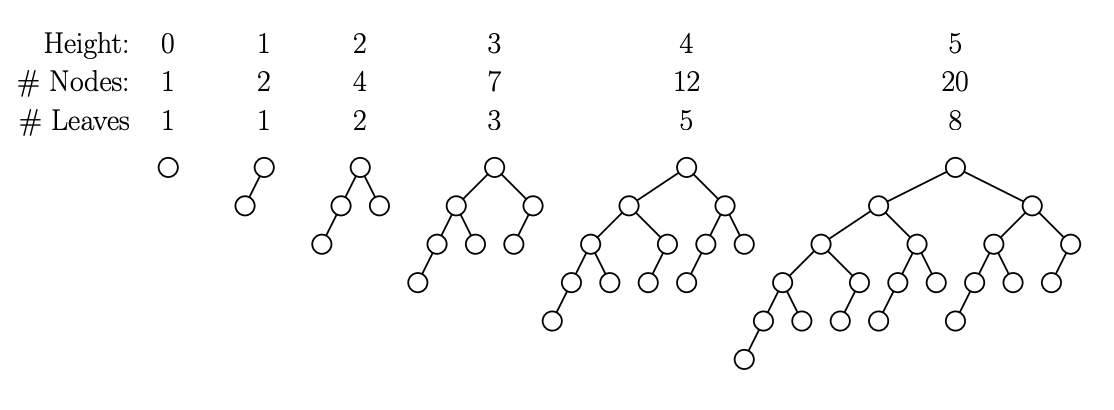
\includegraphics[width=\textwidth]{FibTreeMinNodes}
  Rotations are used to main tree's balance by modifying relation between two nodes but preserving the tree's inorder properties 
  \begin{lstlisting}
    BinaryNode rotateRight(BinaryNode p) {
      BinaryNode q = p.left;
      p.left = q.right;
      q.right = p;
      return q;   // q is now root
    }
    Binary Node rotateLeft(Binary Node p) {
      BinaryNode q = p.right;
      p.right = q.left;
      q.left = p;
      return q;   // q is now root
    }
  \end{lstlisting}
  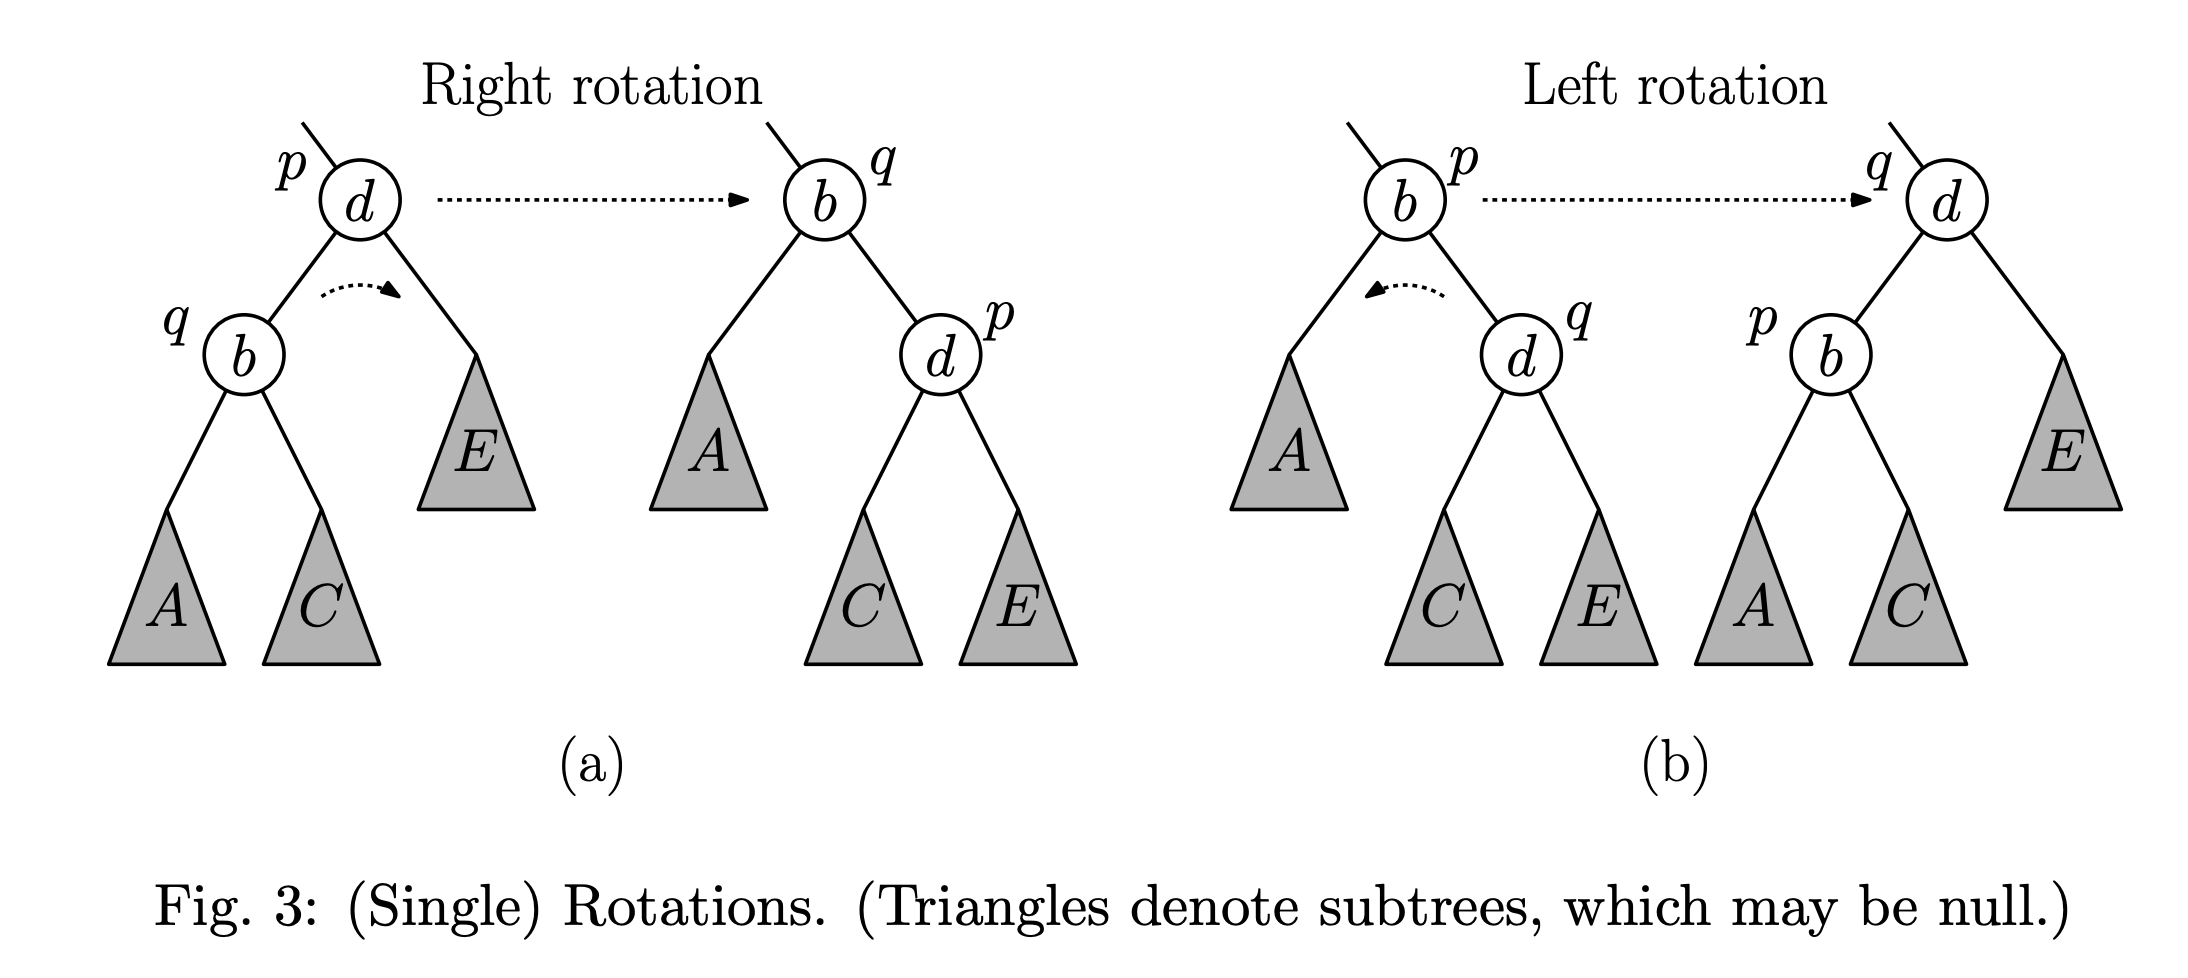
\includegraphics[width=\textwidth]{FibTreeRotation}
  Single rotations work when the imbalance occurs on the outer edges of the tree. Need to use double rotations LR or RL to balance inner trees \\
  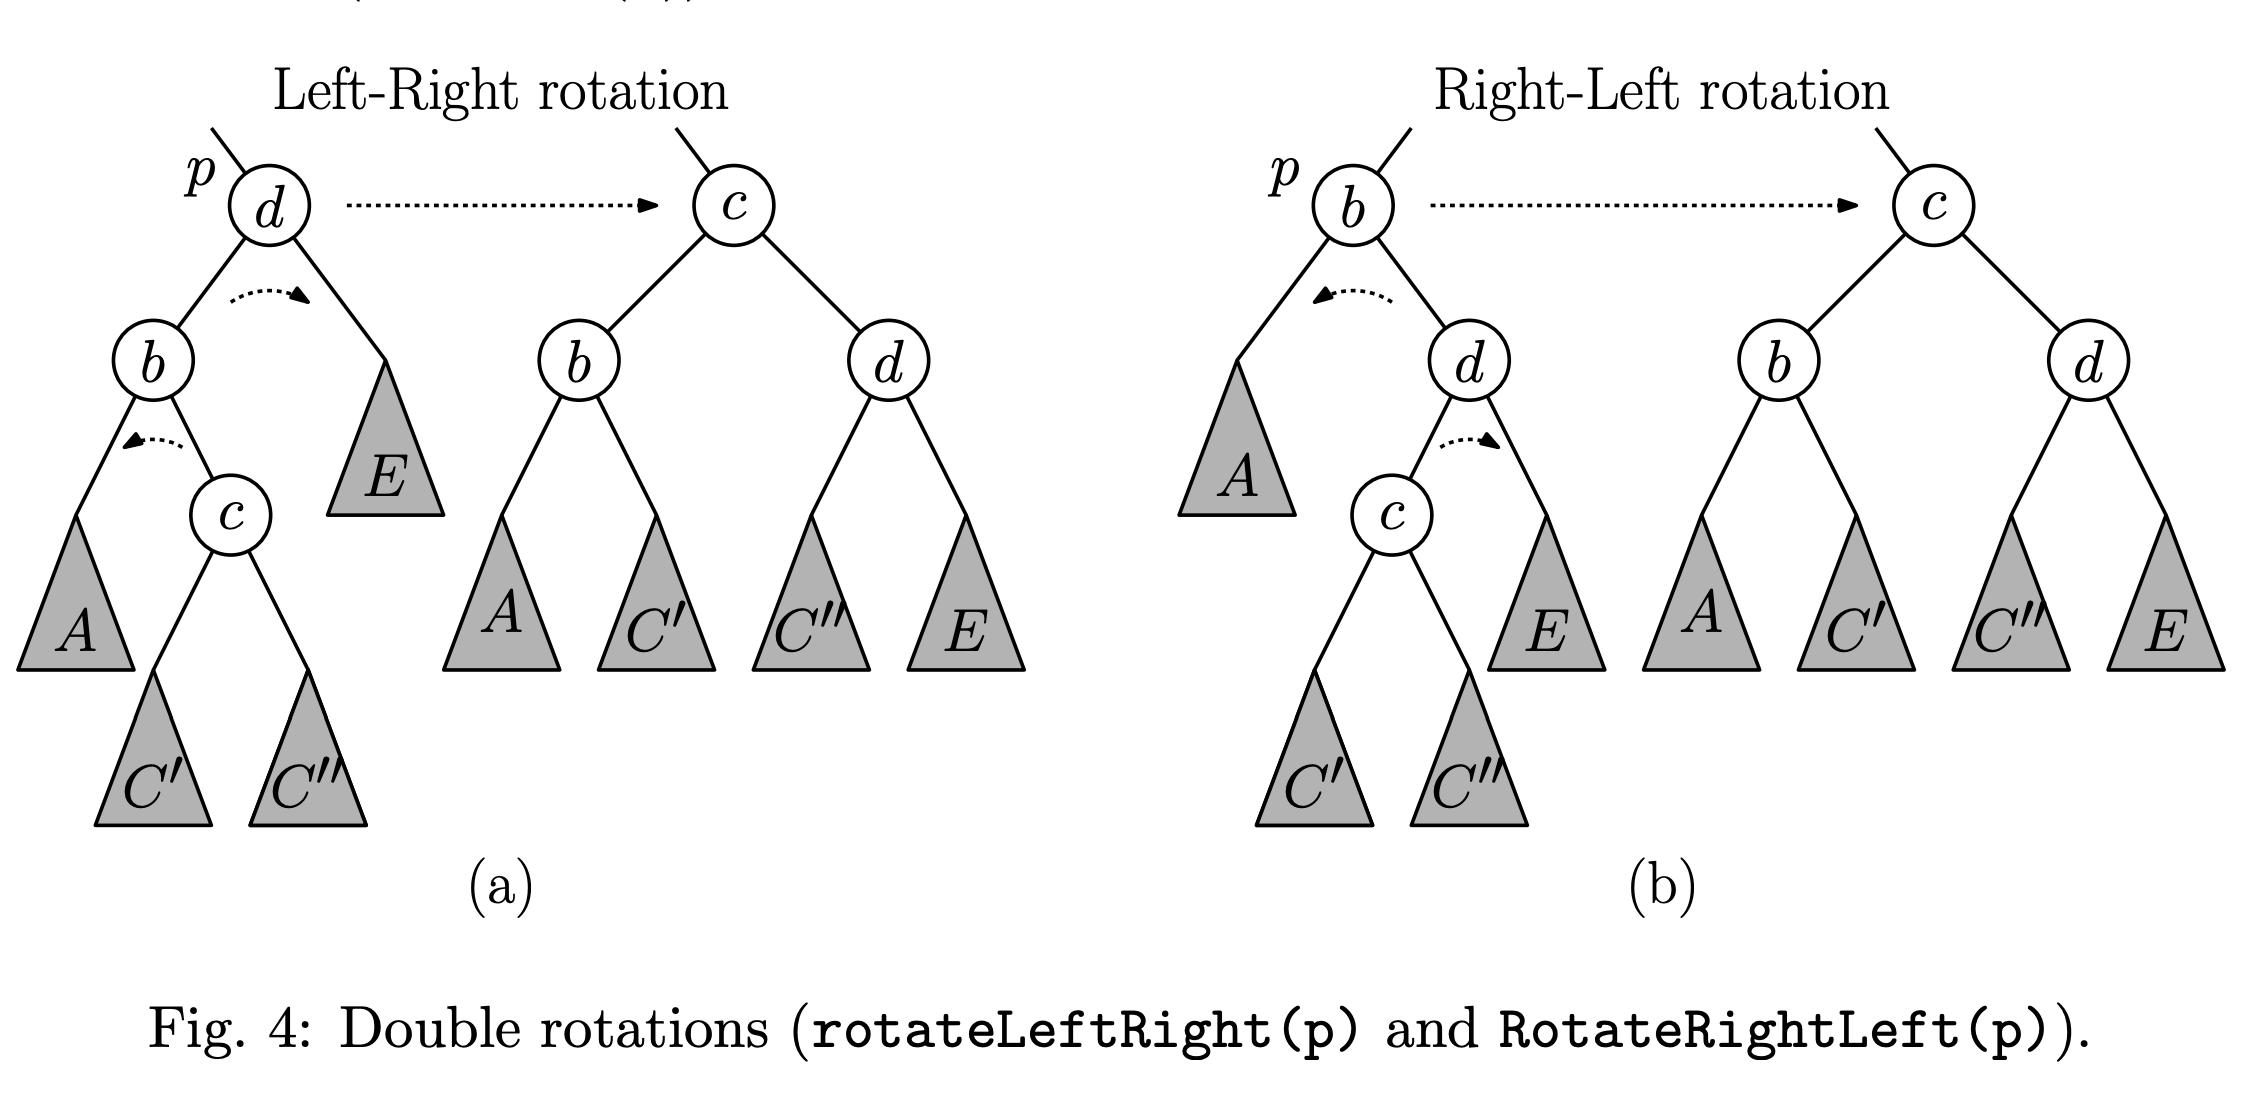
\includegraphics[width=\textwidth]{FibTreeDoubleRotation}
  Insertion works similar to BST except we update the heights of subtrees and apply rotations to maintain height \\
  When insertion occurs balance factors of ancestors is altered by $\pm$1\\
  If a node has a balance factor that violates Balance Property: \\
  \indent Left-Left substree too deep then rotate right \\
  \indent Right-Right subtree too deep then rotate left \\
  \indent Left-Right subtree too deep then rotate left-right \\
  \indent Right-Left subtree too deep then rotate right-left
  \begin{lstlisting}
    int height(AvlNode p) return p == null ? -1 : p.height;
    void updateHeight(AvlNode p) p.height = 1 + max(height(p.left), height(p.right));
    int balanceFactor(AvlNode P) return height.(p.right) - height(p.left);
    AvlNode rotateRight(AvlNode p) {
      AvlNode q = p.left;
      p.left = q.right;   // swap inner child
      q.right = p;        // bring q above p
      updateHeight(p);
      updateHeight(q);
      return q;           // q replaces p
    }
    AvlNode rotateLeft(AvlNode p) {... symmetrical to rotateRight ...}
    AvlNode rotateLeftRight(AvlNode p) {
      p.left = rotateLeft(p.left);
      return rotateRight(p);
    }
    AvlNode rotateRightLeft(AvlNode p) {... symmetrical to rotateLeftRight ...}
    AvlNode insert(Key x, Value v, AvlNode p) {
      if (p == null) p = newAvlNode(x, v, null, null);
      else if (x < p .key) p.left = insert(x, v, p.left);
      else if (x > p.key) p.right = insert(x, v, p.right);
      else throw DuplicateKeyException;
      return rebalance(p);
    }
    AvlNode rebalance(AvlNode p) {
      if (p == null) return p;
      if (balanceFactor(p) < -1) {
        if (height(p.left.left) >= height(p.left.right)) {//left-left heavy
          p = rotateRight(p);
        } else {                                          //left-right heavy
          p = rotateLeftRight(p);
        }
      }
      else if (balanceFactor(p) > 1) {
        if(height(p.right.right) >= height(p.right.left)) {//right-right heavy
          p = rotateLeft(p);
        } else {                                            //right-left heavy
          p = rotateRightLeft(p);
        }
      }
      updateHeight(p);
      return p;
    }
  \end{lstlisting}
  Deletion works in a similar manner in that we call normal BST delete and then rotate as necessary. However we need to call rebalance on further ancestors to check balance condition
\end{document}

